\section{Framework}\label{sec:framework}
The Pandas library provides the user with two main data structures:
a one-dimensional Series and a two-dimensional Dataframe.
To abstractly interpret the Python program with Pandas code, we must define the abstract lattice for both the
Pandas data structures and the basic Python data structures (int, float, list, string, etc.).

The lattice consists of multiple layers with values representing the least amount of information at the top and values
representing more detailed knowledge as we go down the hierarchy.
The Figures~\ref{fig:hierarchy}~and~\ref{fig:upper_part} show how the abstract lattice is defined.

\vspace{-1em} % for smaller gap between figures


\begin{figure}[H]
    \caption{Lower part of the Lattice}
    \label{fig:hierarchy}
    \centering
    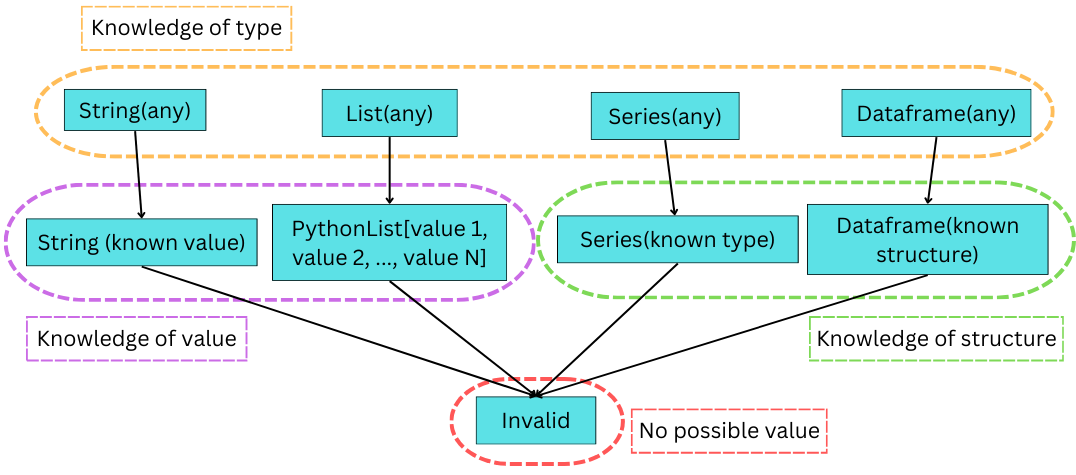
\includegraphics[scale=0.3]{splash_abstract/img/hier}
\end{figure}

\vspace{-2em} % for smaller gap between figures

\begin{figure}[H]
    \caption{Upper part of the Lattice}
    \label{fig:upper_part}
    \centering
    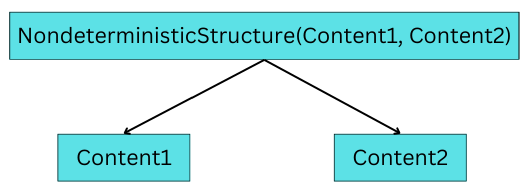
\includegraphics[scale=0.3]{poster/img/nondeterm}
\end{figure}

The Invalid value at the very bottom of the lattice represents a value that we were not able to derive
(usually due to an error in interpretation).
Then there is a level containing full information in the case of Python types, column structure (column types and names)
in the case of Dataframe and the knowledge of the type and label of a Series.
In the next level, there is just partial information --- the type of the structure.
And whenever the interpretation comes to the point when two values are possible, it uses NondeterministicStructure
to represent the uncertainty between the two options.
Such an uncertainty usually occurs in the if-statement.
Other Python types can be added similarly as String and List.